%%% Laboratory	 Notes
%%% Template by Mikhail Klassen, April 2013
%%% Contributions from Sarah Mount, May 2014
\documentclass[a4paper]{tufte-handout}

\newcommand{\workingDate}{\textsc{April $|$ 2022}}
\newcommand{\userName}{A.Belcaid}
\newcommand{\institution}{ENSA-Safi}

\usepackage{lab_notes}

\usepackage{hyperref}
\hypersetup{
    pdffitwindow=false,            % window fit to page
    pdfstartview={Fit},            % fits width of page to window
    pdftitle={Correction TD2},     % document title
    pdfauthor={Your Name},         % author name
    pdfsubject={},                 % document topic(s)
    pdfnewwindow=true,             % links in new window
    colorlinks=true,               % coloured links, not boxed
    linkcolor=DarkScarletRed,      % colour of internal links
    citecolor=DarkChameleon,       % colour of links to bibliography
    filecolor=DarkPlum,            % colour of file links
    urlcolor=DarkSkyBlue           % colour of external links
}


\title{Solution TD 2}
\date{2022}

\begin{document}
\maketitle

%%%%%%%%%%%%%%%%%%%%%%%%%%%%%%%%%%%%%%%%%%%%%%%%%%%%%%%%

\section{Exercice 1}
L'espace d'etats est $\Omega = \left\{ (i,j)\;|\; i\neq j\;,\; 1\leq i,j\leq
n\right\} ou le resultat$ $(i,j)$ represente la position de parking d'Ali et
Najib. Ainsi on applique la loi \textbf{uniforme} pour calculer la probababilite
de l'evenement concerne:
 
\begin{equation*}
  A = \left\{ (i,j) \in \Omega \;|\; \vert i -j \vert \leq 2 \right\}
\end{equation*}

\begin{marginfigure}
    \centering
    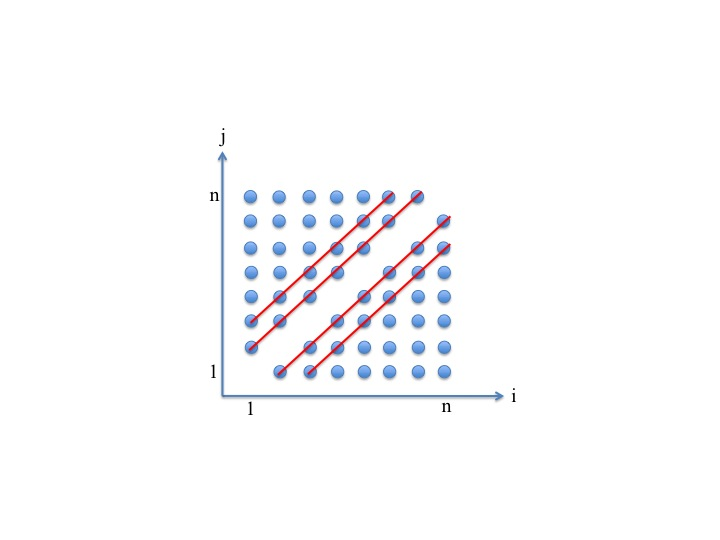
\includegraphics[width=8cm, height=6cm]{figures/exo1_event.jpg}
\end{marginfigure}

On calcule tout d'abord le \textbf{cardinal} de $\Omega$. On possede $n^2$ pairs
$(i,j)$. Cependant une position avec $(i,i)$\footnote{deux voitures ne peuvent
pas parquer dans la meme position.}, le cardinal de $\Omega$ est 
\begin{equation*}
  n^2 - n = n(n-1)
\end{equation*}


On considere tout d'abord le cas ou $n \geq 3$, l'evenement $A$ consiste des
\textbf{quatre} lignes traces dans la figure. Il contient $2(n-1) + 2(n-2) =
4n-6$ elemenets.\\[4pt]

Pour $n=2$, l'evenement $A$ contient seulement les deux elements $(1,2)$ et
$(2,1)$, ce qui est consistent avec la formule $4(2) - 6 = 2$. Ainsi on conclut
que:

\begin{equation*}
  \mathbf{P}(A) = \frac{4n-6}{n(n-1)}
\end{equation*}



\hrule


\section{Calcul de probabilite espace continu}

\begin{enumerate}
  \item Probabilite de $\mathbf{A}$:\\
La figure montre l'espace des etats continu et les regions hachuree
correspondent a l'evenemtn $A$.
\begin{marginfigure}
  \centering
  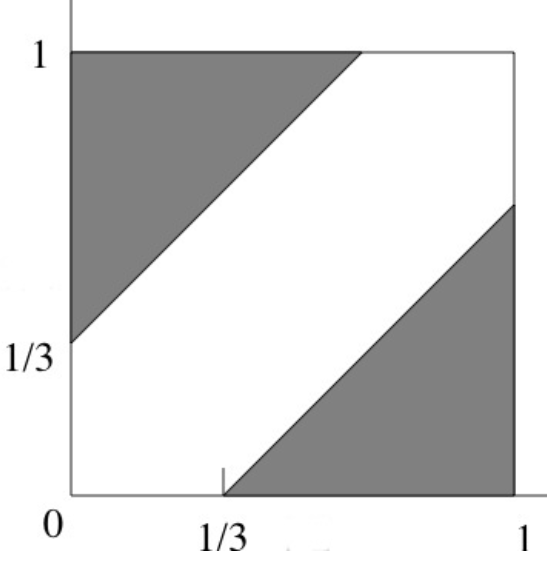
\includegraphics[width=0.8\textwidth]{figures/exo2_1.png}
  \caption{Choix qui differe par plus de $1/3$.}
\end{marginfigure}
Puisqu'il sagit d'une loi de probabilite \textbf{uniforme}, on reduit le calcul
des probabilite auy calcul de la surface.
\begin{equation*}
  \mathbf{P}(A) = 2\cdot \frac{\left(\frac{2}{3}\right)^2}{2} = \frac{4}{9}
\end{equation*}
\item Probabilite de $\mathbf{B}$:\\
  L'ensemble qui correspond a $B$ est trace dans la figure suivante:

\begin{marginfigure}
  \centering
  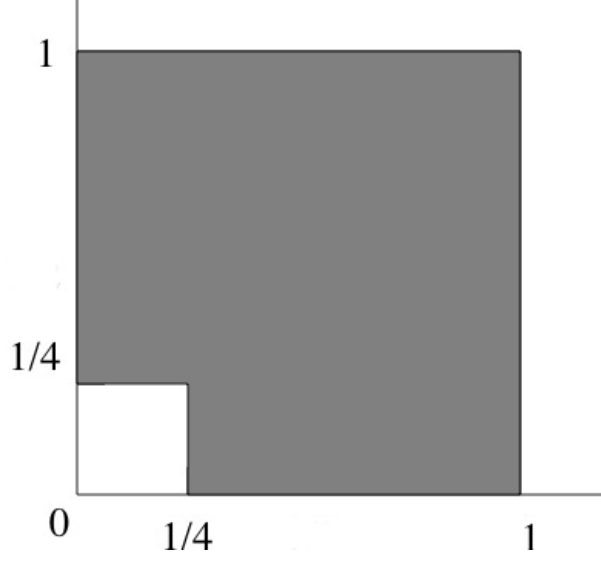
\includegraphics[width=0.8\textwidth]{figures/exo2_2.png}
  \caption{Les deux superieurs a  $1/4$.}
\end{marginfigure}
Ainsi la probabilite est egale:

\begin{eqnarray*}
  \mathbf{P}(B) &=& 1 - \mathbf{P}(B^c) \\
                &=& 1 - \frac{1}{4}\frac{1}{4}\\
                &=& \frac{15}{16}
\end{eqnarray*}
\item Probabilite de $\mathbf{C}$:\\
  La figure montre la region qui correspond a $C$.
\begin{marginfigure}
  \centering
  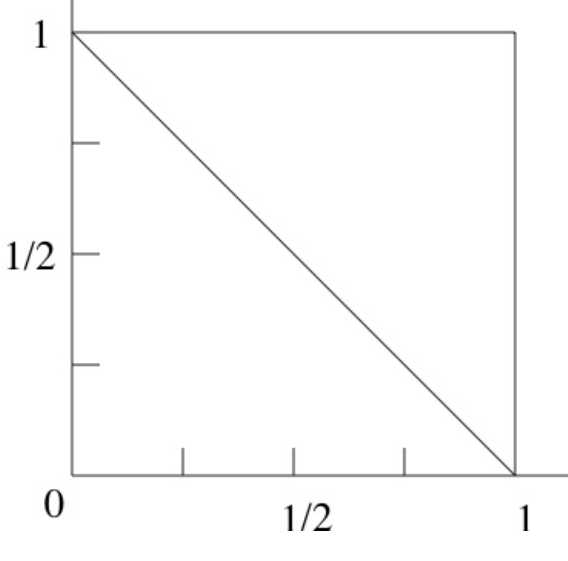
\includegraphics[width=0.8\textwidth]{figures/exo2_3.png}
  \caption{Region $x + y = 1$.}
\end{marginfigure}

\begin{equation*}
\mathbf{P}(C) = \int_0^1dx \int_{1-x}^{1-x}dy = 0
\end{equation*}

\item La probabilite de l'evenement $\mathbf{D}$:\\

\begin{marginfigure}
  \centering
  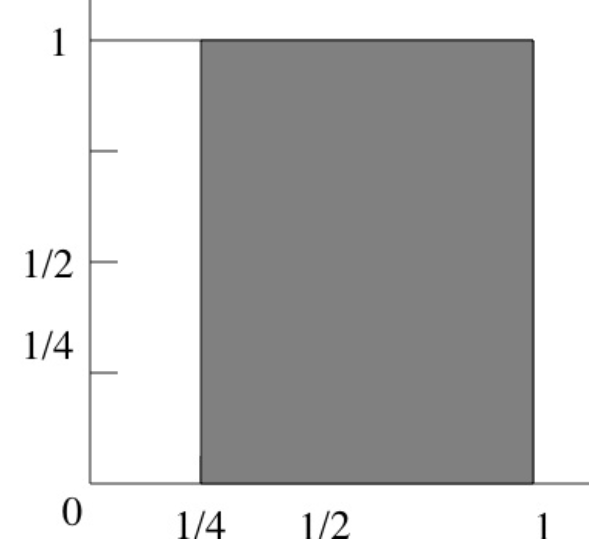
\includegraphics[width=0.8\textwidth]{figures/exo2_4.png}
  \caption{Region $x \geq \frac{1}{4}$.}
\end{marginfigure}

\begin{equation*}
  \mathbf{P}(D) = 1\cdot \frac{ 3}{4}  = \frac{3}{4}
\end{equation*}

\item Probabilite de $A\cap D$:\\

\begin{marginfigure}
  \centering
  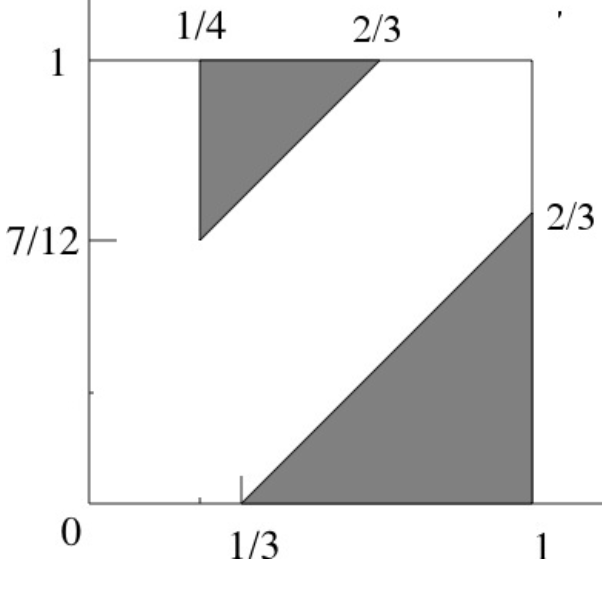
\includegraphics[width=0.8\textwidth]{figures/exo2_5.png}
  \caption{Region d'intersection entre A et D.}
\end{marginfigure}

\begin{equation*}
  \mathbf{P}(A\cap D) = \frac{2}{3}\cdot\frac{2}{3}\cdot \frac{1}{2} +
  \frac{5}{12}\cdot\frac{5}{12}\cdot \frac{1}{2} = \frac{89}{288}
\end{equation*}


\end{enumerate}

\hrule

\section{Inegalite de Benferroni}

\begin{enumerate}
  \item Regle pour \textbf{deux evenements}:\\
    \begin{equation*}
    \mathbf{P}(A_1 \cap A_2) \geq \mathbf{P}(A_1)  + \mathbf{P}(A_2)
    \end{equation*}
    On a:

    \begin{eqnarray*}
      \mathbf{P}\left(\left(A_1\cap A_2\right)^c\right) &=&
      \mathbf{P}\left(A_1^c  \cup A_2^c\right)  \leq \mathbf{P}(A_1^c) +
      \mathbf{P}(A_2^c)\\
      1 - \mathbf{P}(A_1 \cap A_2) &\leq & 1 - \mathbf{P}(A_1^c)  + 1 -
      \mathbf{P}(A_2^c)\\
      \mathbf{P}(A_1 \cap A_2) &\geq& \mathbf{P}(A_1) + \mathbf{P}(A_2) - 1
    \end{eqnarray*}

  \item \textbf{Generalisation}:
    \begin{equation*}
      \mathbf{P}(A_1\cap \ldots \cap A_n) \geq \mathbf{P}(A_1) + \ldots +
      \mathbf{P}(A_n) - (n-1)
    \end{equation*}
\end{enumerate}
\begin{itemize}
  \item \textbf{Cas Initial} : Pour $n=2$ c'est deja demontre dans la premiere
    question.
  \item \textbf{Heredite}:  On suppose que la relation est vrai pour $n-1$ et on
    la demontre pour $n$.
    \begin{eqnarray*}
      \mathbf{P}(\underbrace{A_1\cap \ldots }_{B}\cap A_n)& \geq& \mathbf{P}(B) +
      \mathbf{P}(A_n) - 1 \\
                                                          &\geq &
                                                          \mathbf{P}(A_1) +
                                                          \ldots +
                                                          \mathbf{P}(A_{n-1}) -
                                                          (n-2) +
                                                          \mathbf{P}(A_n) - 1\\
                                                      & \geq & \mathbf{P}(A_1) + \ldots +
      \mathbf{P}(A_n) - (n-1)
    \end{eqnarray*}
\end{itemize}

%%\newpage
\bibliographystyle{plain}
 % \bibliography{lab_notes}

\end{document}
